\documentclass{ULBreport}

\sceau{Pictures/official_logos/sceauULB.png}

\addbibresource{biblio.bib}


%%glossary and acronyms package

\usepackage[toc,acronyms]{glossaries}

\usepackage{float}

\usepackage{eurosym}

\makeglossaries

% \newglossaryentry{strip mining}
% {
%   name=strip mining,
%   description={is the practice of mining a seam of mineral, by first removing a long strip of overlying soil and rock}
% }



% \newacronym{t}{t}{tons}



\begin{document}

\titleULB{
	title={Two bars and one elastic},
	course={Control System Design},
	author={Emmeran COLOT},
	date={2024},
	teacher={Prof. Emanuele Garone},
	logo={Pictures/official_logos/logos.jpg}
}

\listoftables % ToC for tables

\listoffigures % ToC for figures

\setcounter{secnumdepth}{-1}

\chapter{Introduction}

\section{Context}

We have been tasked to design a numeric controller for a given system which has to meet some requirements. The system is 
called \textit{DC motor and brake} and it consists of two current controlled motors connected to a brake trough a shaft. \\

Our objective is to send the best signal to the motors to ensure that:

\begin{enumerate}
    \item[$\bullet$] the shaft can reach any reasonnable speed in less than half a second
    \item[$\bullet$] the shaft's speed in maintained as smooth as possible
    \item[$\bullet$] the system can reject a step disturbance as fast as possible
    \item[$\bullet$] the shaft's speed can follow a feasible speed reference of $4 Hz$ from any feasible speed
\end{enumerate}

In addition to this, we could implement a strategy to reject various brake disturbances profile and magnitude, while 
maintaining the speed variations as smooth as possible.

\section{Plant description}

As explained in the introduction, the plant consists of two motors and one brake acting on the same shaft. There are 
three sensors available: one speed sensor and two position sensors.

\begin{figure}[H]
    \centering
    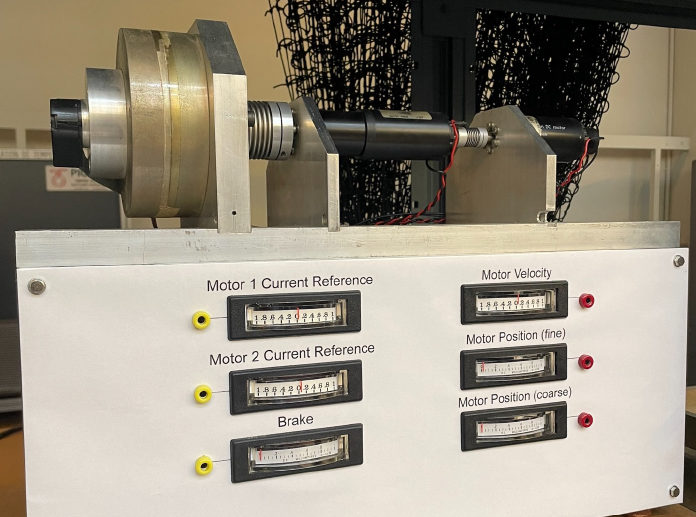
\includegraphics[height=\textheight/5]{Pictures/plant_picture.png}
    \caption{Picture of the plant}
\end{figure}



\setcounter{secnumdepth}{2}

\chapter{System identification}
\label{section:identification}

\section{Derivation of the System Dynamics}

To analyze the transfer function of a system with two DC motors and a brake using current-driven dynamics, we incorporate the relationships between motor current, torque, and angular velocity. Using Newton's Second Law for rotational dynamics, we determine the torque balance on the shaft. The system's dynamics are described by the following mechanical equations:

\begin{itemize}
    \item \textbf{DC Motors:} The motors are current-driven, meaning the torque produced by each motor is proportional to the input current:
    \begin{equation}
        T_m = K I
        \label{eq:dc_motor_eq}
    \end{equation}
    
    \item \textbf{Brake:} The brake applies a frictional torque that opposes the rotation of the shaft. This braking torque is often modeled as proportional to the shaft velocity:
    \begin{equation}
        T_b = c_b \omega
        \label{eq:brake_eq}
    \end{equation}
    
    \item \textbf{Torque Balance on the Shaft:} The shaft's angular velocity is proportional to the net torque on the shaft. The frictional torque is given by:
    \begin{equation}
        T_f = b \omega, \quad \text{where } T_f \text{ is the friction torque.}
        \label{eq:shaft_eq_friction}
    \end{equation}
    The total torque balance equation is:
    \begin{equation}
        T_s + T_f = T_m - T_b
        \label{eq:shaft_eq}
    \end{equation}
    Substituting \eqref{eq:dc_motor_eq}, \eqref{eq:brake_eq}, and \eqref{eq:shaft_eq_friction} into \eqref{eq:shaft_eq}, we obtain:
    \begin{equation}
        J \frac{d\omega}{dt} + b \omega + c_b \omega = K I
        \label{eq:shaft_eq_final}
    \end{equation}
    
    \item \textbf{Electrical Dynamics:} Applying Kirchhoff's Voltage Law to the motor circuit:
    \begin{equation}
        L\frac{d i}{dt} + R i = V - K \omega
        \label{eq:dc_motor_eq_final}
    \end{equation}
    where \( e = K \omega \) in \eqref{eq:dc_motor_eq_final} is the back EMF, proportional to the angular velocity of the motor shaft.
\end{itemize}

Taking the Laplace transform of the equations:

1. For the torque balance on the shaft:
\begin{equation}
    J s \Omega(s) + (b + c_b) \Omega(s) = K I(s)
    \label{eq:shaft_eq_final_laplace}
\end{equation}

2. For the electrical dynamics:
\begin{equation}
    L s I(s) + R I(s) = V(s) - K \Omega(s)
    \label{eq:Kirchhoff_eq_final_laplace}
\end{equation}

By eliminating \( I(s) \), the transfer function relating the output (rotational speed of the shaft) \( \Omega(s) \) to the input voltage \( V(s) \) is derived:
\begin{equation}
    G(s) = \frac{\Omega(s)}{V(s)} = \frac{K}{(J s + b + c_b)(L s + R) + K^2}
    \label{eq:2nd_st_order_TF}
\end{equation}

This describes the dynamic response of the DC motor, where the rotational speed is expressed in rad/sec per volt of input.

\section{Characteristics of the Transfer Function}
Based on the mechanical equations of the DC motor, the 2nd-order system can be simplified to a first order system to reduce complexity and mitigate the effects of noise and friction variations. By making reasonable assumptions, the transfer function is linearized and approximated to match the expected form of a first-order system transfer function, which is already known as:

\begin{equation}
    G(s) = \frac{A_0}{\tau s + 1}
    \label{eq:1_st_order_TF}
\end{equation}

Because it has no pole in $0$ (or equivalently it is a non-integrator system), the response of the system to a step
command is enough to find both $A_0$ and $\tau$.\\

As the plant is not perfect (the motors have some friction variations depending on the temperature, there is noise, 
\dots), the objective is to establish a linearized model of it. In the following section, the determination of a
transfer function for motor 1 will be explained in detail. This transfer function will link the speed of the shaft to
the voltage applied to motor 1. We only study the speed and not the position because all of the requirements are on
the speed, meaning that there is no point of studying the position.

\section{Step response}

The starting point of the step response experiment is the static characteristic of the motor:

\begin{figure}[H]
    \centering
    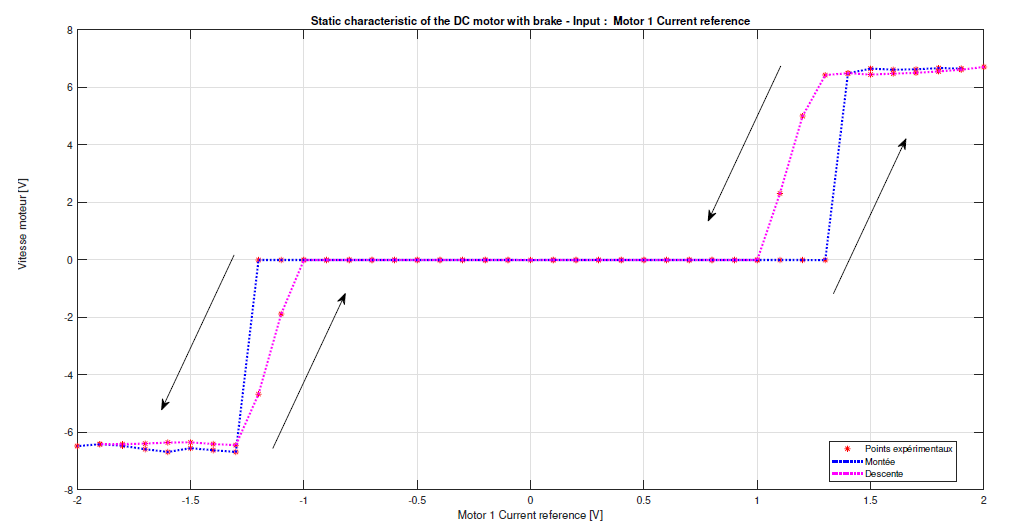
\includegraphics[height=\textheight/4]{Pictures/static_characteristic_motor_1.png}
    \caption{Static characteristic of the system driven by the motor 1}
    \label{fig:static_characteristic_motor_1}
\end{figure}

By analyzing figure \ref{fig:static_characteristic_motor_1}, a first obvious deduction to be made is that the velocity
cannot reach a value greater than approximately $6.5 V$\footnote{Any speed will be expressed in volts ($V$) as speed is
measured by a sensor that returns a voltage} (and $-6.5 V$ is minimum value). This clarifies the use of "\textit{
feasible}" in the requirements as a speed of $7 V$ could never been achieved, no matter what the input is.\\

What is really interesting to understand is that the static characteristic gives the speed of the shaft after a
sufficient amount of time (in theory, after an infinite amount of time but in practice, once the transient response 
vanishes). By looking at it, it is clear that to have a speed that is different from $0 V$ and that is outside of the
saturated region, a high command should be sent to reach saturation and it must then be lowered to a point where the
speed is no longer saturating (a command between $1.1 V$ and $1.3 V$ approximately).\\

With this in mind, the following step response has been recorded:

\begin{figure}[H]
    \centering
    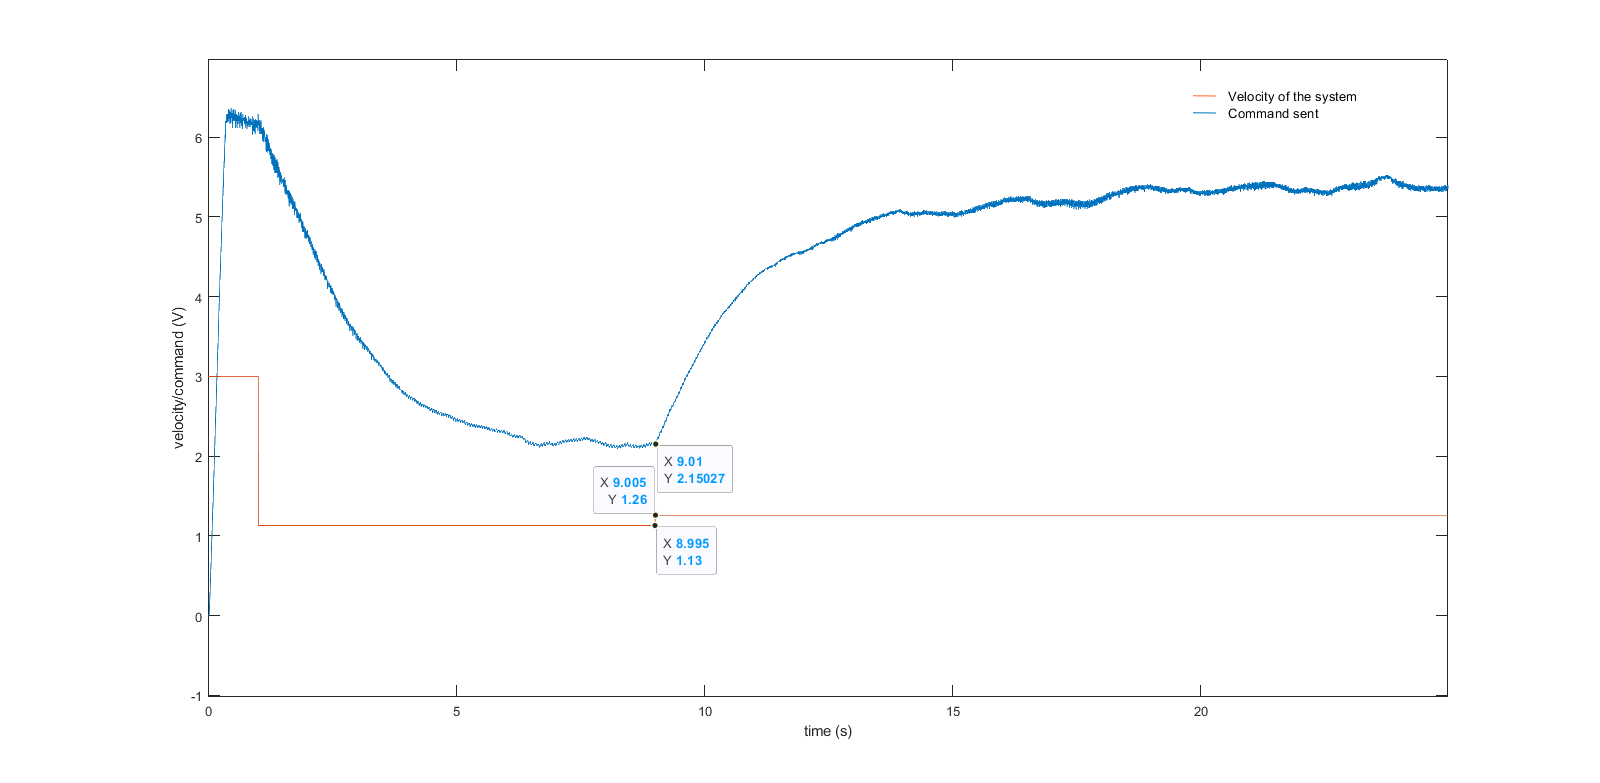
\includegraphics[height=\textheight/3]{Pictures/step_response_positive_motor_1.png}
    \caption{Step response of the system when the motor 1 has a step as command}
    \label{fig:step_response_positive_motor_1}
\end{figure}

%%NOT GOOD

Where the command is first set at a high enough voltage ($\geq 1.5 V$, based on \ref{fig:static_characteristic_motor_1}). 
After the velocity saturates, it lowers to a value where the velocity will stabilize ($1.13 V$). This operating point 
\textit{$OP_{1+}$} will correspond to the transfer function $G(s)$ that we are trying to estimate here. Then the step is
introduced (with a magnitude of $0.13 V$).

\begin{equation}
    OP_{1+} = \begin{bmatrix}
        \text{command} = 1.13 V \\
        \text{velocity} = 2.15 V
    \end{bmatrix}
\end{equation}

With a coordinates change for easier visualization, the data plot \ref{fig:estimated_step_response_positive_motor_1} is 
used for the determination of $A_0$ and $\tau$. It is indeed known that for a transfer function in the form of 
\ref{eq:1_st_order_TF}, the parameter $A_0$ is equal to the asymptotic value of the step response divided by the amplitude 
of the step. $\tau$ on the other hand is equal to the time after which the step response reaches $\frac{e-1}{e}$ ($\approx 0.63$)
times the asymptotic step response. This gives as transfer function:

\begin{equation}
    G_{1+}(s) = \frac{24.88}{1.915s + 1}
    \label{eq:TF_mot1_+}
\end{equation}

The name $G_{1+}(s)$ has been chosen because the "\textit{$1$}" indicates that it corresponds to the motor 1 and the 
"\textit{$+$}" indicates that it is used for a positive speed. As shown on the static characteristic 
\ref{fig:static_characteristic_motor_1}, the operating point at which the system will be operating to have a negative speed 
($OP_{1-}$) is quite far from $OP_{1+}$, which means that another model will be needed to describe the behavior of the 
system in this zone (see discussion in section \ref{section_validation}).\\

With the model \ref{eq:TF_mot1_+}, the simulated step response can be computed and as shown in figure 
\ref{fig:estimated_step_response_positive_motor_1} it can be seen that it matches quite well with the experimental results.

\begin{figure}[H]
    \centering
    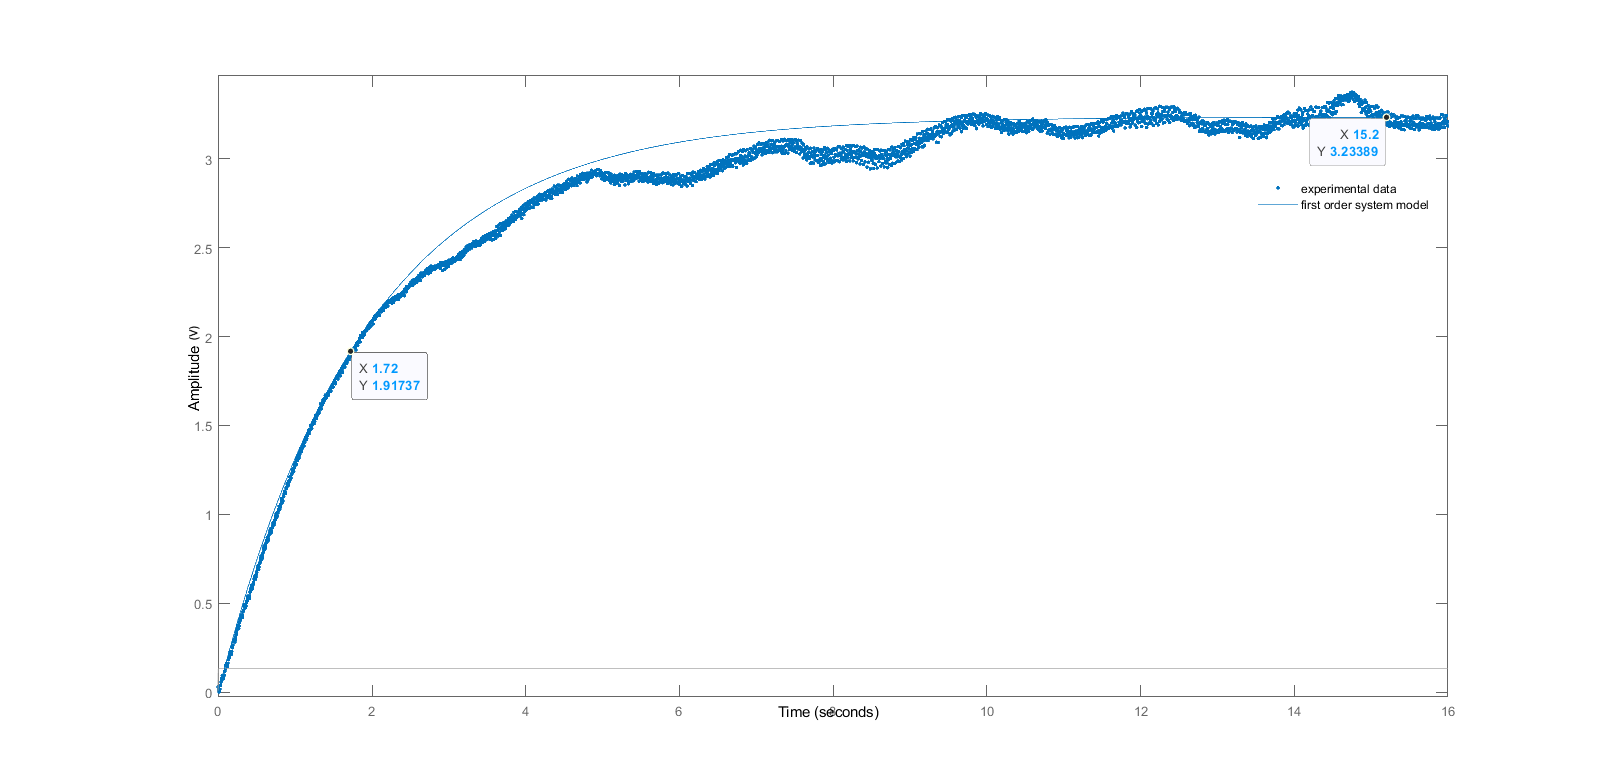
\includegraphics[height=\textheight/3]{Pictures/first_order_model_positive_motor_1.png}
    \caption{Estimation of the step response compared to the real one}
    \label{fig:estimated_step_response_positive_motor_1}
\end{figure}

\section{Validation}
\label{section_validation}

The estimated transfer function established in section \ref{section:identification} must yet be tested. Indeed, as it
is the result of the linearization of the real plant around the equilibrium point $OP_{1+}$ we have to ensure that it
has the same behaviour as the plant even when the system is not in $OP_{1+}$.\\

The system has been controlled by a step similar to the one in figure \ref{fig:step_response_positive_motor_1} with slightly
modified values. It started at $1.2 V$ and the downward step has been chosen with an amplitude of $0.05 V$. Figure 
\ref{fig:validation_A0_24} shows the step command with the real plant response and the response computed based on the
transfer function \ref{eq:TF_mot1_+}.

\begin{figure}[H]
    \centering
    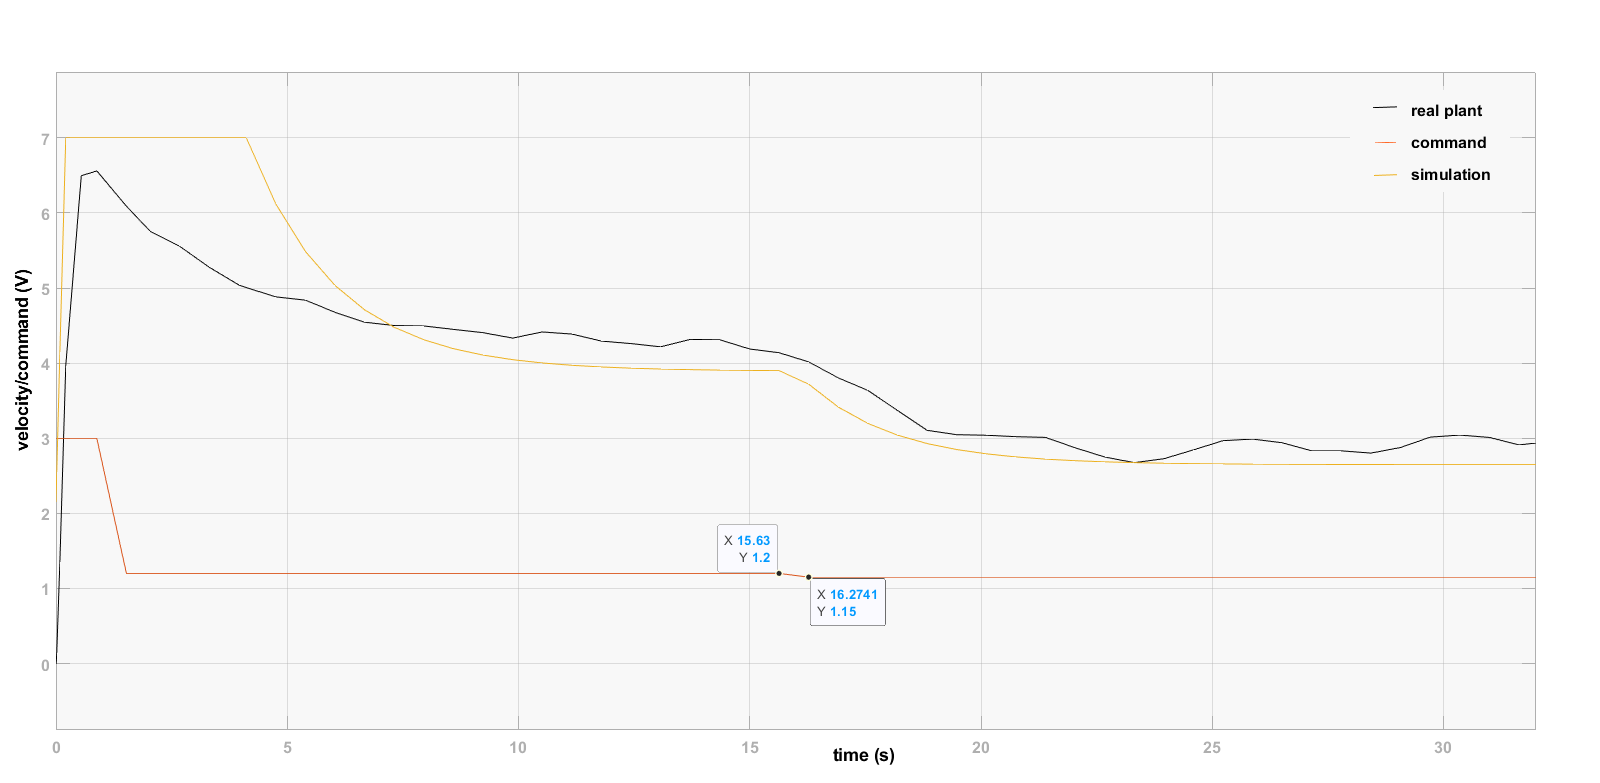
\includegraphics[height=\textheight/3]{Pictures/validation_A0_24.png}
    \caption{Validation of the model $G_{1+} (s)$}
    \label{fig:validation_A0_24}
\end{figure}

It appears quite clearly that the simulated response is not corresponding to the real one. Note that the first part of
the response (until $\sim 10s$) is not interesting as the model does not have to take the velocity saturation into account.
Based on the observation that the asymptotic value of the velocity was not corresponding between the real plant and the
simulation, we tried changing $A_0$ to get a better matching. With $A_0 = 30$, the model was close to the reality as 
shown in figure \ref{fig:validation_A0_30}, which leads to the transfer function:

\begin{equation}
    \tilde{G}_{1+}(s) = \frac{30}{1.915 s + 1}
\end{equation}

The conclusion that can be drawn from this whole section is that depending on the operating point, the transfer function
needs to be modified \textit{by a multiplicative factor} but the position of the pole does not change. This means that 
$G_{1+}(s)$ can be used if we keep in mind that the numerator can vary a little.

\begin{figure}[H]
    \centering
    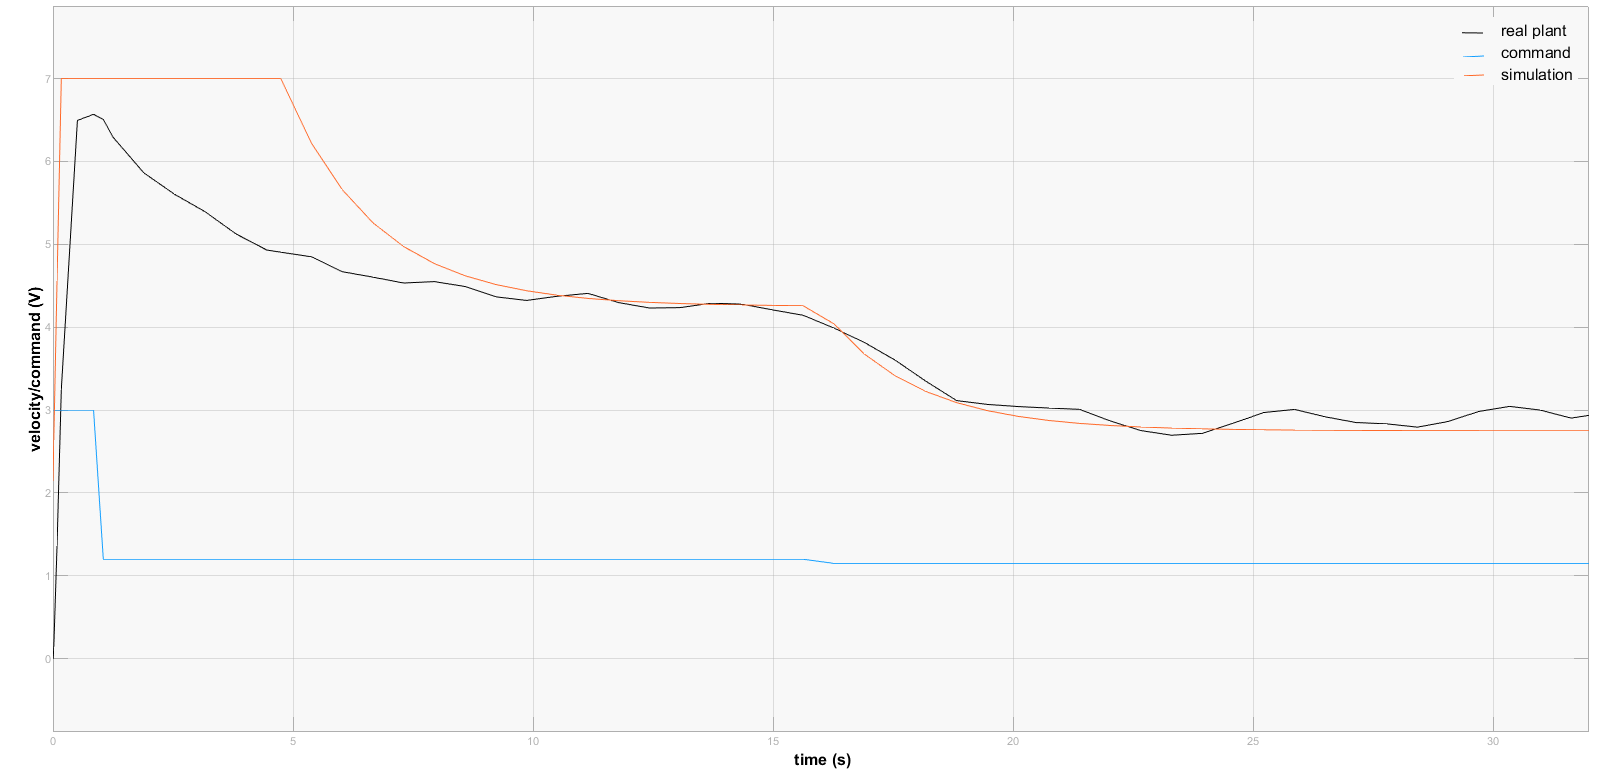
\includegraphics[height=\textheight/3]{Pictures/validation_A0_30.png}
    \caption{Validation of the modified model $\tilde{G}_{1+}(s)$}
    \label{fig:validation_A0_30}
\end{figure}

\section{Other transfer functions}

Based on the same experiment, we determined the other transfer functions\footnote{With the naming convention mentioned 
before}:

\begin{align}
    G_{1-}(s) &= \frac{24.31}{1.85 s + 1} & OP_{1-} &= \begin{bmatrix}
                \text{command} & = & -1.1 V \\
                \text{velocity} & = & -1.494 V
                \end{bmatrix} 
    \label{TF_mot1_-} \\
    G_{2+}(s) &= \frac{19.51}{1.7 s + 1} & OP_{2+} &= \begin{bmatrix}
                \text{command} & = & 1.1 V \\
                \text{velocity} & = & 2.4 V
                \end{bmatrix} 
    \label{TF_mot2_+} \\
    G_{2-}(s) &= \frac{26.86}{2.09 s + 1} & OP_{2-} &= \begin{bmatrix}
                \text{command} & = & -1.1 V \\
                \text{velocity} & = & -2.51 V
                \end{bmatrix} 
    \label{TF_mot2_-}
\end{align}




\setcounter{secnumdepth}{1}

\chapter{Design of the controller}

\section{Requirements analysis}

The first step of the controller design is to analyse the requirements that have been given in the introduction:

\begin{enumerate}
    \item[$\bullet$] the shaft can reach any reasonable speed in less than half a second
    \item[$\bullet$] the shaft's speed in maintained as smooth as possible
    \item[$\bullet$] the system can reject a step disturbance as fast as possible
    \item[$\bullet$] the shaft's speed can follow a feasible speed reference of $4 Hz$ from any feasible speed
\end{enumerate}

There is one reference tracking objective, one disturbance rejection objective and two dynamical response properties.
The design of the controller will follow the following path:

\begin{enumerate}
    \item Rejecting a step disturbance (with each motor separately)
    \item Following a $4 Hz$ reference (with each motor separately)
    \item Merge the two controllers into a single digital one
    \item Reach any speed in $< 0.5 s$
\end{enumerate}

The method used here is to design the controller in the Laplace domain in the first time. Once the continuous time
controller has the desired behaviour, it is discretized using the Tustin method (without forgetting to take the
ZOH into account).

\section{Disturbance rejection}

From theory, it is known that a controller is able to asymptotically reject a disturbance if it has at the denominator
of its transfer function the denominator of the disturbance.\\

As a step disturbance is of the form:

\begin{equation}
    D(s) = \frac{A e^{-\tau s}}{s}
\end{equation}

The controller will need a pole in $0$. This can be easily done by using a PI controller, which looks like:

\begin{align}
    C_{PI}(s) &= k_p \left( 1 + \frac{1}{T_i s} \right)\\
    &= k_p \left(\frac{T_i s + 1}{T_i s} \right)
    \label{eq:general_PI}
\end{align}

The $k_p$ will be chosen once the dynamic response characteristics will have to be met. However, $T_i$ can already be 
chosen based on a simple criteria. As the open-loop transfer function equals the product $C_{PI}(s) \times G_{1+} (s)$, a
solid choice is to use $T_i$ to cancel the pole in the system. This way, the position of the poles of the closed-loop
will be entirely based on the controller.\\
Of course this will be true in the case of a perfect model but as proved in the section \ref{section_validation}, the
parameter $\tau$ of the transfer function (which fixes the pole of it) don't seems to move a lot depending on the 
operating point. We can conclude from this that the best choice is:

\begin{equation}
    T_i = \tau
\end{equation}

for each controller, which leads to:

\begin{equation}
    C_{PI}(s) = k_p \left( \frac{\tau s + 1}{\tau s} \right) 
    \label{eq:controller_PI}
\end{equation}


\iffalse
\section{Reference tracking}

For tracking purposes, the method used to reject disturbances can also be applied. Indeed, a reference with $D(s)$ at
its denominator will be perfectly followed if the controller denominator contains $D(s)$.

\begin{align}
    R(s) &= \mathcal{L}\left\{A \sin (8 \pi t + \varphi)\right\} \\
    &= \frac{8 A \pi e^{-\frac{\varphi s}{8 \pi}}}{s^2 + (8\pi)^2}
\end{align}

A second controller is needed to ensure the tracking of a $4 Hz$ sine:

\begin{equation}
    C_{\sin}(s) = \frac{1}{s^2 + (8\pi)^2}
    \label{eq:controller_sin}
\end{equation}

This controller has no parameter that can be moved as we chose a minimalist controller. 
\fi

\section{Frequential analysis}
\label{section:freq_analysis}

As the next objective is to perfectly track a $4 Hz$ reference, the bandwidth of the closed loop has to be studied. If
it is greater than $4 \times 2\pi \approx 25$, then there is no need to add a part to the controller's structure.\\
The bandwidth is determined using the Bode curves of the closed loop. This means that the structure of the regulator
has to be defined. In continuous time, it looks like:

\begin{figure}[H]
    \centering
    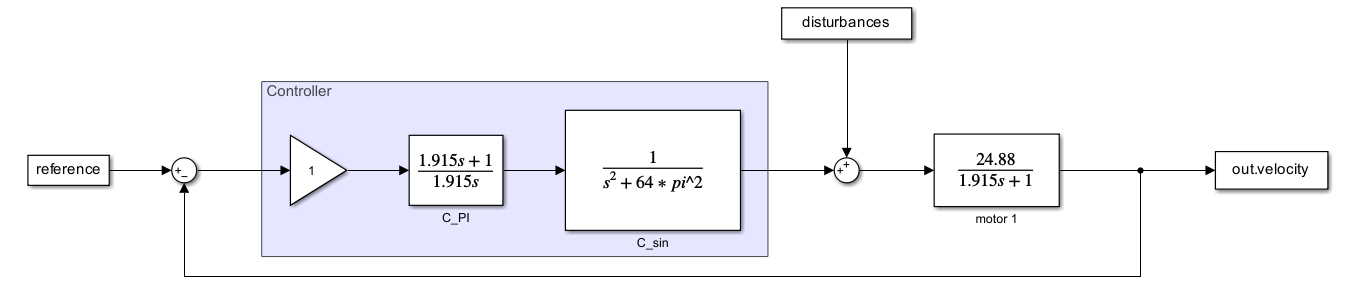
\includegraphics[height=\textheight/7]{Pictures/controller_structure.png}
    \caption{Structure of the closed loop system with a PI regulator}
    \label{fig:CL structure}
\end{figure}

To determine the gain (= $k_p$) that can be put in the system, the \texttt{margin} method of matlab is used (fig 
\ref{fig:OL bode}) on the open-loop transfer function with $k_p$ set to 1. A gain margin of $6 dB$ has to be maintained 
\footnote{by convention} to ensure the stability of the system once the loop is closed. \\

\begin{figure}[H]
    \centering
    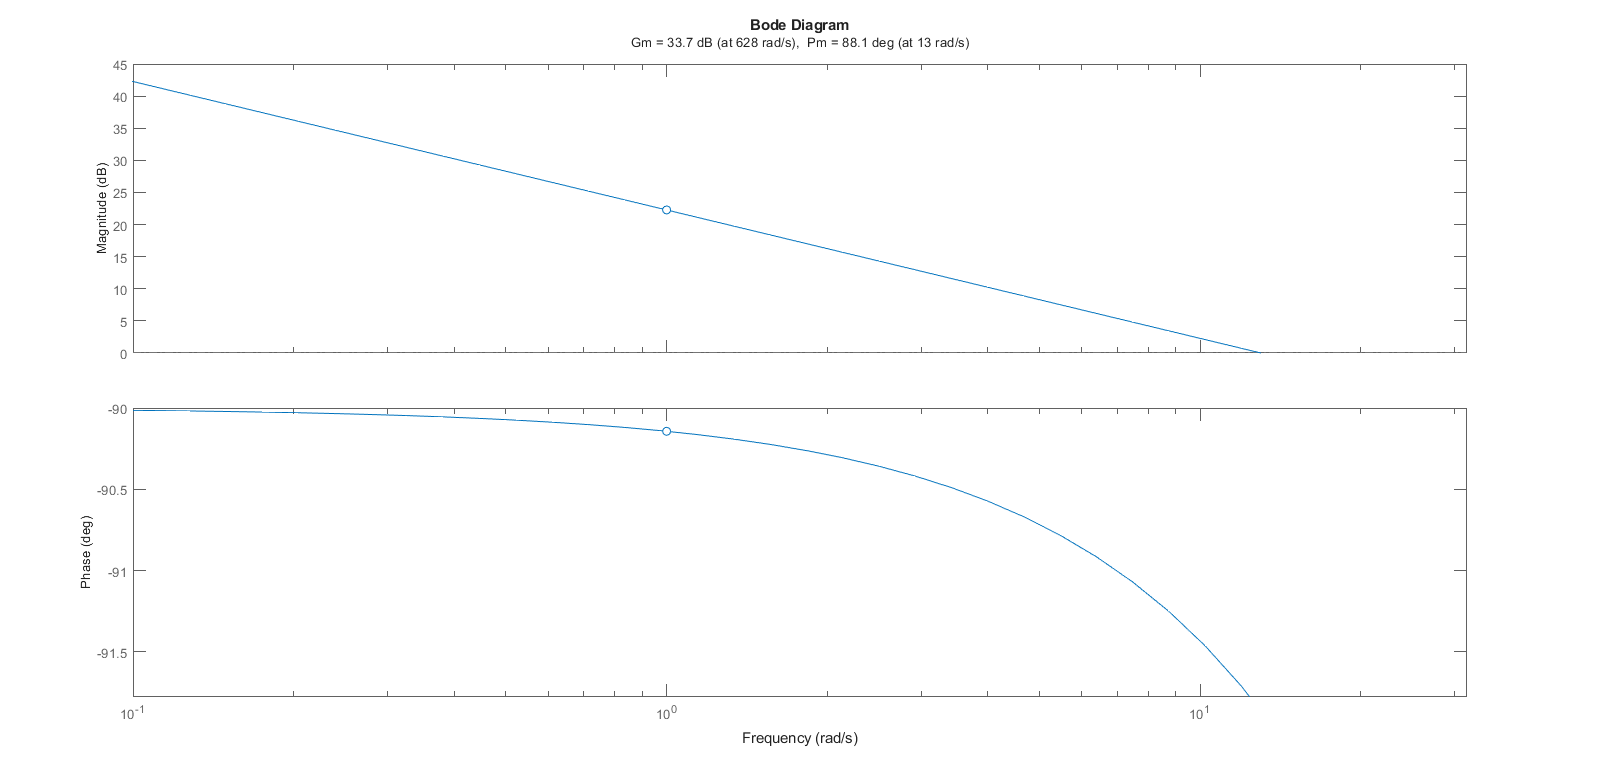
\includegraphics[height=\textheight/3]{Pictures/bode_OL.png}
    \caption{Bode diagram of the open loop system with the stability margins}
    \label{fig:OL bode}
\end{figure}

To keep a gain margin of at least $6 dB$, we can multiply $k_p$ (which was set to 1) by $27.7 dB = 10^{27.7/20} = 24.26$
. This means that if the loop is closed with $k_p = 24$, the closed loop system will be stable and it's bandwidth can
be determined. This is done by taking the frequency at which the gain of the closed loop system falls under $-3 dB$.\\ 
Figure \ref{fig:CL bode} gives a bandwidth of around $709 \text{rad}/s$. However to be more realistic and also to stay 
with a small phase (as it reaches $-200 ^{\circ}$ when the magnitude is $-3 dB$), the "\textit{safe}" bandwidth is $111 
\text{rad}/s$. This proves that a simple PI controller is sufficient to perfectly track a signal at $4 Hz$.

\begin{figure}[H]
    \centering
    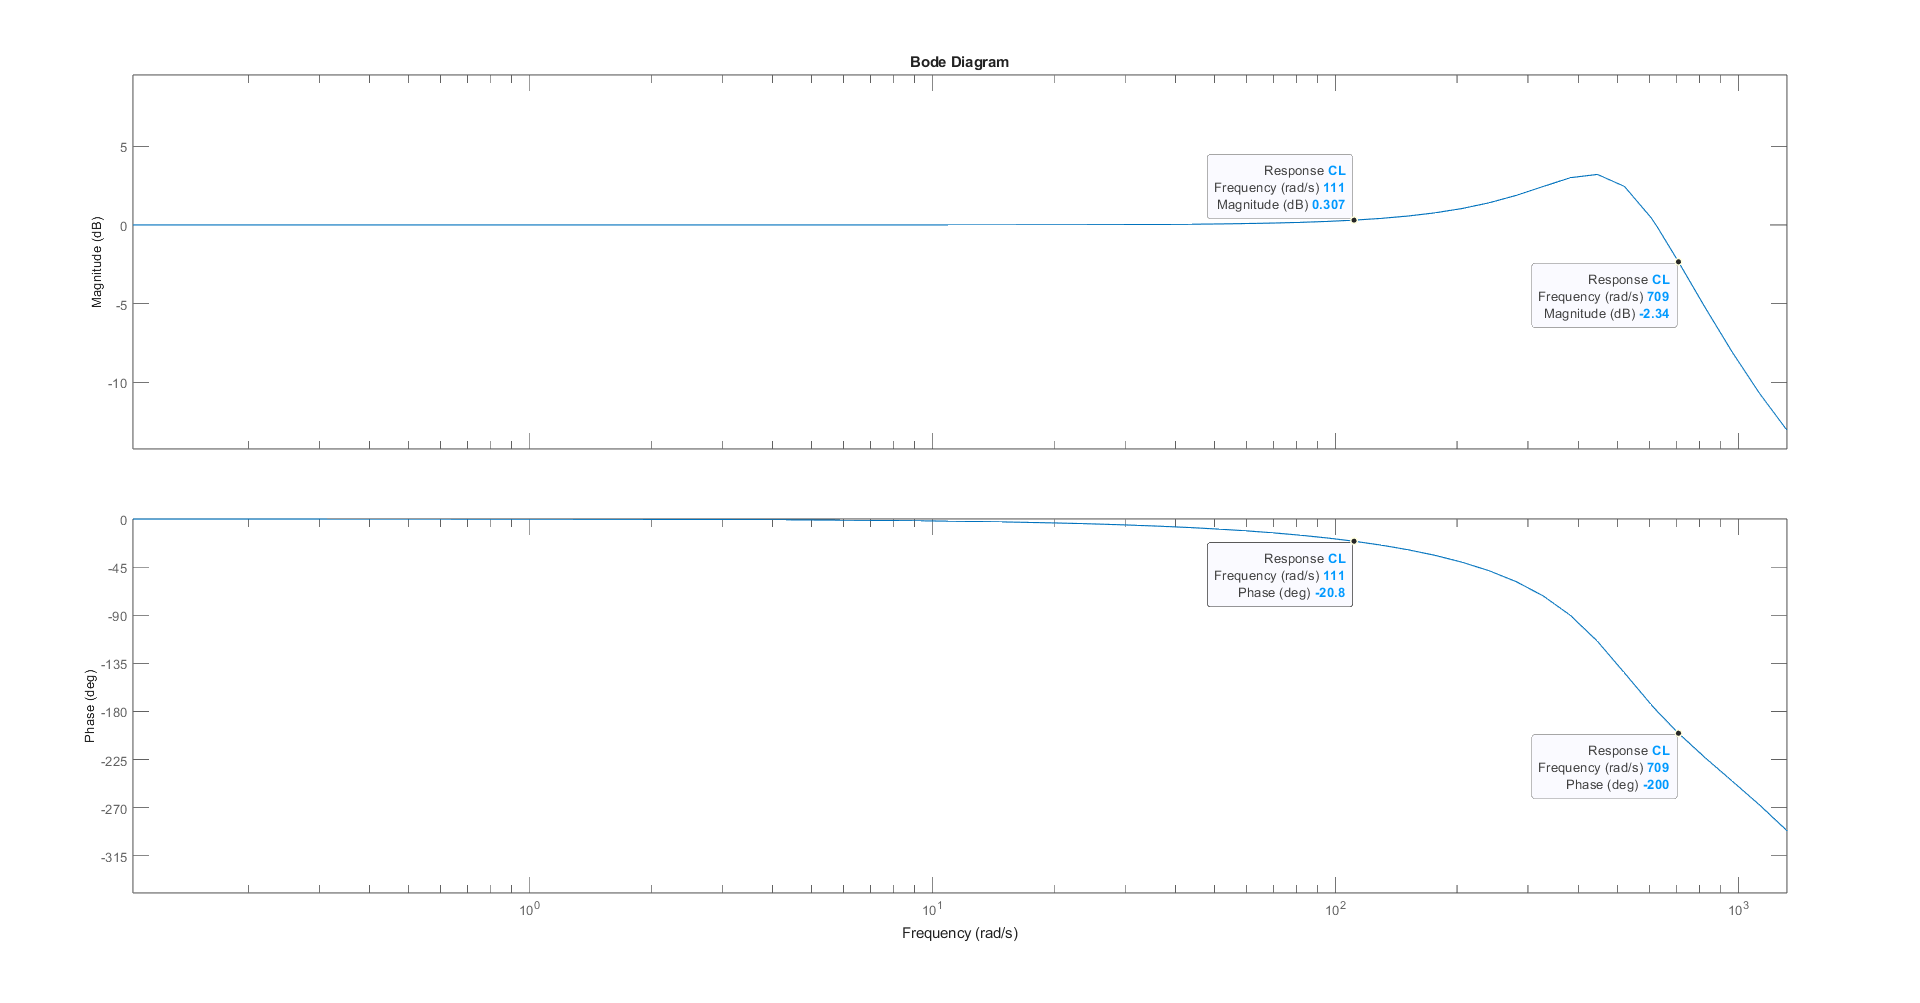
\includegraphics[height=\textheight/3]{Pictures/bode_CL.png}
    \caption{Bode diagram of the closed loop system for $k_p = 24$}
    \label{fig:CL bode}
\end{figure}



\chapter{LQR Controller}

\section{State Space Model}
In control system design, it is often easier to define a parameterized state-space model in continuous time because 
physical laws are typically described using differential equations. The linear state-space representation in 
continuous-time has the following form:

\begin{equation}
    \dot{\mathbf{x}} = A \mathbf{x} + B \mathbf{u}
    \label{eq:state_space_models}
\end{equation}

where \( \mathbf{x} \) is the state vector, \( A \) is the state matrix that represents the system dynamics, 
\( B \) is the input matrix that represents the control input, and \( \mathbf{u} \) is the input vector.\\
To get to the state space representation from the transfer function is quite easy as each motor is a $1^{st}$ order
system. By using the following property of the Laplace transform:

\begin{align}
    X(s) &= \mathcal{L}\left\{x(t)\right\}\\
    s X(s) &= \mathcal{L}\left\{\frac{d x(t)}{dt}\right\}
\end{align}

The transfer function \ref{eq:1_st_order_TF} can be put in the temporal domain:

\begin{align}
    G(s) = \frac{Y(s)}{U(s)} &= \frac{A_0}{\tau s + 1}\\
    \left(\tau s + 1\right) Y(s) &= A_0 U(s)\\
    \tau \dot{y}(t) + y(t) &= A_0 u(t)\\
    \dot{y}(t) &= \frac{-1}{\tau} y(t) + \frac{A_0}{\tau} u(t)
\end{align}

This can be done for both motors with respectively ($u_1/y_1$) and ($u_2/y_2$) as input and output. With the choice of 
state $x_i(t) = y_i(t)$, the state space representation becomes

\begin{equation}
    \dot{\mathbf{x}}(t) = \begin{bmatrix}
    \frac{-1}{\tau_1} & 0 \\ 
    0 & \frac{-1}{\tau_2}
    \end{bmatrix} \mathbf{x}(t) + \begin{bmatrix} 
    \frac{A_{01}}{\tau_1} \\ 
    \frac{A_{02}}{\tau_2} 
    \end{bmatrix}\mathbf{u}(t)
    \label{eq:state_space_model_cx}
\end{equation}

\begin{equation}
    y(t) = \begin{bmatrix} 1 & 1 \end{bmatrix}\mathbf{x}(t)
    \label{eq:state_space_model_cy}
\end{equation}

where \( y \) is the velocity output.

\section{Discrete-Time State-Space Model}
We convert the continuous-time state-space model \eqref{eq:state_space_model_cx} and \eqref{eq:state_space_model_cy} to 
a discrete-time state-space model using the parameters:

\[
\tau_1 = 1.915, \quad \tau_2 = 1.7, \quad A_{01} = 24.88, \quad A_{02} = 19.51.
\]

The continuous-time matrices are computed as:

\[
\mathbf{A} = 
\begin{bmatrix}
-0.5218 & 0 \\
0 & -0.5882
\end{bmatrix}, \quad 
\mathbf{B} = 
\begin{bmatrix}
12.9870 \\
11.4765
\end{bmatrix}.
\]

For a sampling time \( T_s = 0.1 \, \text{seconds} \), the discrete-time matrices \( A_{T_s} \) and \( B_{T_s} \) are calculated as follows:

\begin{itemize}
    \item \textbf{Discrete-Time State Matrix} (\(A_{T_s}\)): 
   Using the matrix exponential formula:
   \[
   A_{T_s} = e^{A T_s},
   \]
   where:
   \[
   A T_s = 
   \begin{bmatrix}
   -0.05218 & 0 \\
   0 & -0.05882
   \end{bmatrix}.
   \]
   Since \( A T_s \) is a diagonal matrix, the matrix exponential is computed as:
   \[
   e^{A T_s} = 
   \begin{bmatrix}
   e^{-0.05218} & 0 \\
   0 & e^{-0.05882}
   \end{bmatrix}.
   \]
   Evaluating the exponentials gives:
   \[
   e^{-0.05218} \approx 0.9491, \quad e^{-0.05882} \approx 0.9429.
   \]
   Therefore, we find:
   \[
   A_{T_s} = 
   \begin{bmatrix}
   0.9491 & 0 \\
   0 & 0.9429
   \end{bmatrix}.
   \]
\end{itemize}

\begin{itemize} 
    \item \textbf{Discrete-Time Input Matrix} (\(B_{T_s}\)): 
   Using the formula:
   \[
   B_{T_s} = \int_0^{T_s} e^{A \zeta} B \, d\zeta,
   \]
   and solving numerically, we find:
   \[
   B_{T_s} = 
   \begin{bmatrix}
   1.2662 \\
   1.1149
   \end{bmatrix}.
   \]
\end{itemize}

Thus, the discrete-time state-space representation of the system is:

\[
x[k+1] = A_{T_s} x[k] + B_{T_s} u[k],
\]
\[
y[k] = C x[k],
\]

where:

\[
A_{T_s} = 
\begin{bmatrix}
0.9491 & 0 \\
0 & 0.9429
\end{bmatrix}, \quad
B_{T_s} = 
\begin{bmatrix}
1.2662 \\
1.1149
\end{bmatrix}, \quad
C = 
\begin{bmatrix}
1 & 1
\end{bmatrix}.
\]

Finally, the sampled system is equivalent to a discrete-time system with these matrices. We will now use this representation to design an LQR controller for the given discrete-time system.

\section{LQR Design for Discrete-Time System}

The goal of the Linear Quadratic Regulator (LQR) is to minimize the quadratic cost function:

\[
J = \sum_{k=0}^\infty \left( x[k]^\top Q x[k] + u[k]^\top R u[k] \right).
\]

The weighting matrices \( Q \) and \( R \) must be selected based on system requirements:

\begin{itemize}
    \item \( Q \): Penalizes state deviations, typically represented as a diagonal matrix, e.g., \( Q = \text{diag}(q_1, q_2) \).
    \item \( R \): Penalizes large control efforts, usually a positive scalar, \( R > 0 \).
\end{itemize}

For our design, we assume the following weighting matrices:

\[
Q = \begin{bmatrix}
10 & 0 \\
0 & 1
\end{bmatrix}, \quad R = 1.
\]

The Discrete-Time Algebraic Riccati Equation (DARE) is given by:

\[
P = A_{T_s}^\top P A_{T_s} - \left(A_{T_s}^\top P B_{T_s} \right) 
\left(R + B_{T_s}^\top P B_{T_s} \right)^{-1} 
\left(B_{T_s}^\top P A_{T_s} \right) + Q.
\]

The optimal feedback gain matrix \( K \) is computed as:

\[
K = \left( R + B_{T_s}^\top P B_{T_s} \right)^{-1} \left(B_{T_s}^\top P A_{T_s} \right).
\]

The LQR controller generates the optimal control input:

\[
u[k] = -K x[k],
\]

where \( K \) is the gain matrix, that will be computed using MATLAB.

\subsection*{LQR Feedback Law}
The two motors share control effort based on these gains. If the shaft angular velocities are \( w_{1} \) and \( w_{2} \), then the control law is:

\[
u[k] = -K x[k], \quad u_{1} = -K_{1} w_{1}, \quad u_{2} = -K_{2} w_{2}.
\]

The computation results yield:

\[
K = \begin{bmatrix}
0.6618 \\ 0.0548
\end{bmatrix}, \quad u_{1} = 0.6618 w_{1}, \quad u_{2} = 0.0548 w_{2}.
\]


\setcounter{secnumdepth}{-1}

\chapter{Conclusion}

In conclusion, we were able during the lab sessions to build the two types of controller that are the most used in the industry: PID's and LQR controllers. We reached the objective that were set and we learned with practice what has been seen during the lectures of Pr. Garone.


\appendix

\section{Annex A : tracking outside of the bandwidth}
\label{annex:tracking}

If the requirements were to track a signal at a frequency higher than the bandwidth of the closed loop, two things could 
have been done. Either we increase the bandwidth or we add a specific part to the controller for it to be effective 
around the desired frequency.

\subsection{Lead compensator}

\begin{align}
    H_{\text{lead}}(s) = \frac{s - z_1}{s - p_1} && z_1 < p_1
\end{align}

A widely used type of regulator is the lead compensator. Its principle is easy to understand thanks to the asymptotic
plot of Bode curves. As the zero comes before the pole, the gain plot will be increasing at this point and the pole is 
just there to ensure causality. The zero must be placed where the amplitude of the transfer function must be increased. 
On the other hand, the pole simply has to be placed far enough to not decrease it where it needs to be high. Here is the 
Bode plot for the closed loop with the zero placed in $600 \text{rad}/s$ (where the magnitude started decreasing) 
and the pole in $1000 \text{rad}/s$:

\begin{figure}[H]
    \centering
    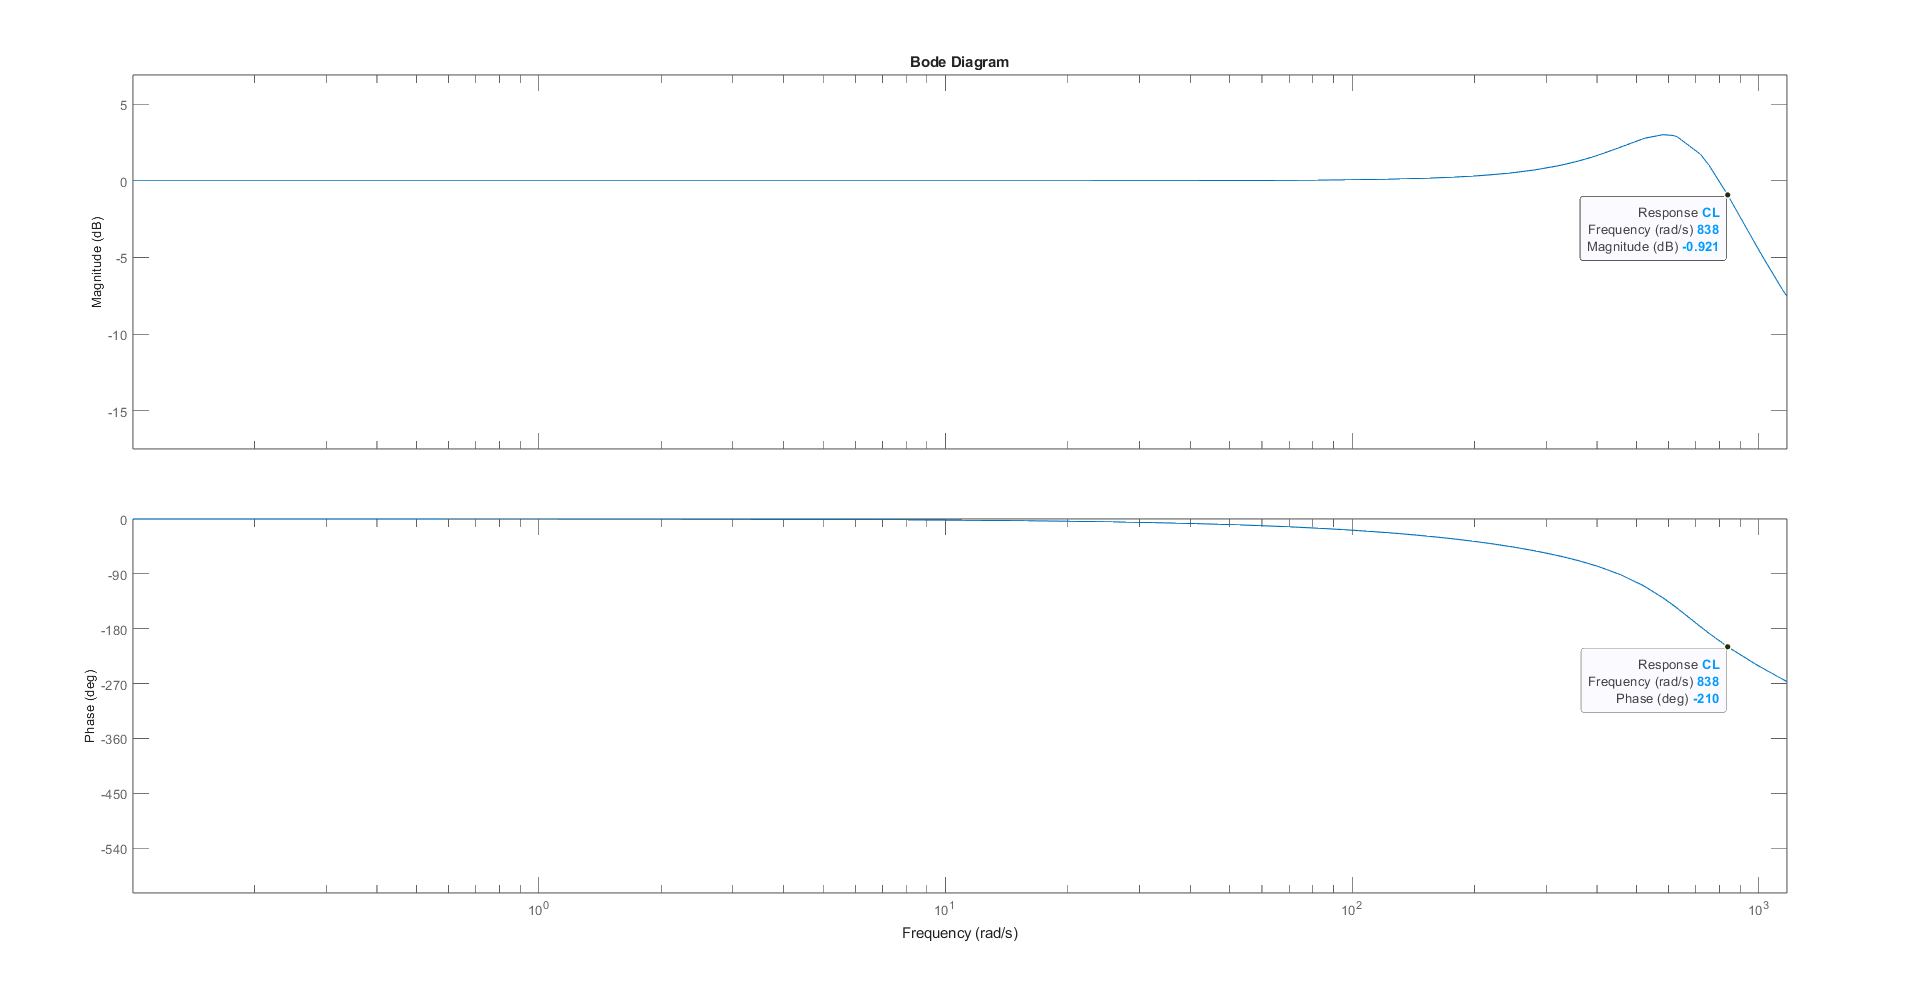
\includegraphics[height=\textheight/3]{Pictures/annex_lead_comp.png}
    \caption{Bode diagram of the closed loop system with a lead compensator $H_{\text{lead}}(s) = \frac{s-600}{s-1000}$}
\end{figure}

This way, the bandwidth has been increased to more than $850 \text{rad}/s$, which is not a significant improve but it
still allows the tracking of faster references.

\subsection{Specific frequency tracker}

\begin{equation}
    H_{\text{spec}}(s) = \frac{1}{s^2 + \omega_{\text{spec}}^2}
\end{equation}

From a theoretical point of view, this regulator is supposed to track perfectly a sine (or cosine) at the pulsation
$\omega_{\text{spec}}$ as it has the same denominator as the reference. However, this transfer function has pure 
imaginary poles. This means that the closed loop system is unstable, despite it having the desired behaviour based on
the Bode plot (magnitude close to $0 dB$ in $\omega_{\text{spec}}$):

\begin{figure}[H]
    \centering
    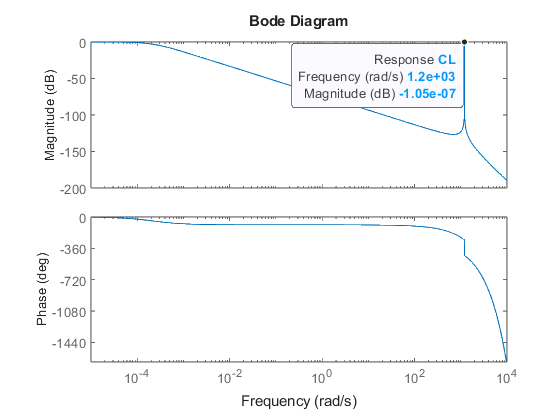
\includegraphics[height=\textheight/3]{Pictures/annex_spec_im.png}
    \caption{Bode diagram of the closed loop system with a specific frequency tracker $H_{\text{spec}}(s) = \frac{1}{s^2
    +1200^2}$}
\end{figure}

It is however really interesting to slightly move these poles away from the imaginary axis and by considering the 
following controller:

\begin{align}
    C(s) &= C_{PI}(s) \times H_{\text{spec}}(s)\\
    &= k_p\times\frac{\tau s + 1}{\tau s(s^2+s+(1200)^2)}
\end{align}

By then following the same methodology as in section \ref{section:freq_analysis}, $k_p = 24\times 10^6$ allows a gain 
of $6 dB$ and the closed loop bandwidth reaches $1300 \text{rad}/s$ as it can be seen on figure 
\ref{fig:spec_ref_tracker}. As this is only an annex, we will stop the analysis here even if this would certainly be 
problematic due to saturation phenomenons\footnote{A simulink simulation would probably prove it}. 

\begin{figure}[H]
    \centering
    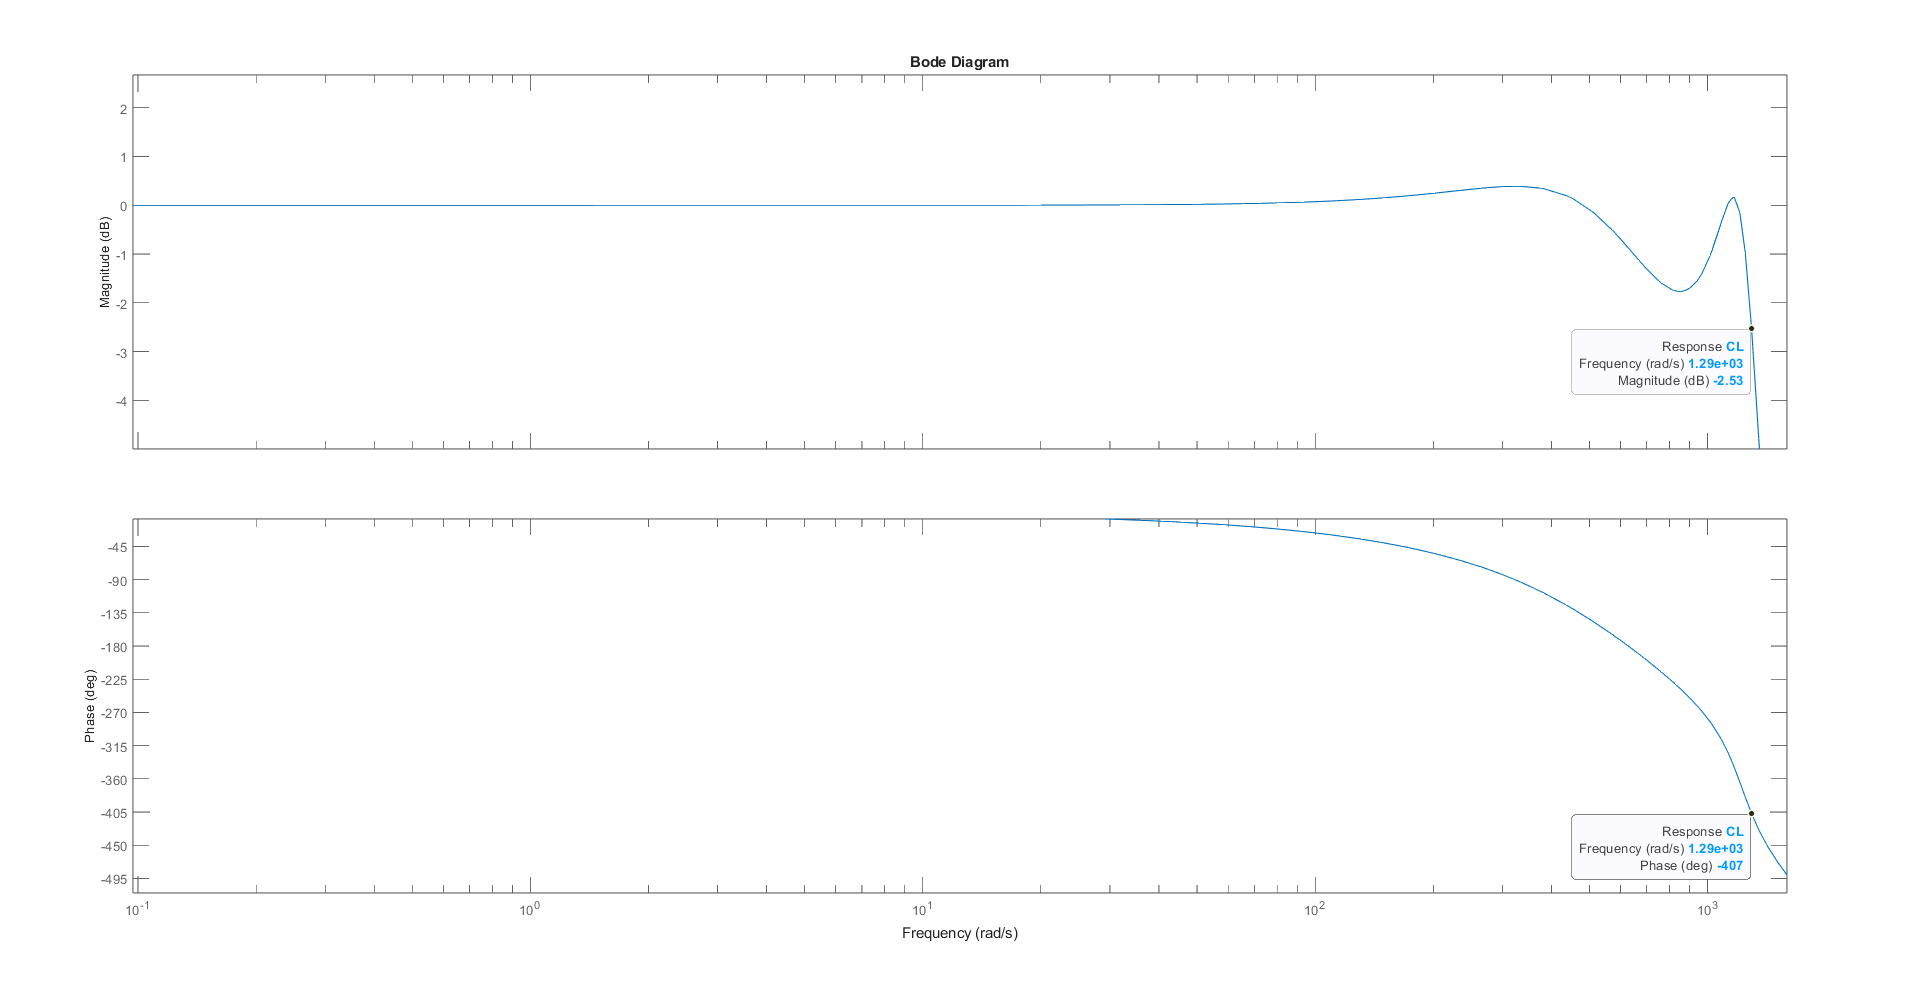
\includegraphics[height=\textheight/3]{Pictures/annex_spec_cmplx.png}
    \caption{Bode diagram of the closed loop system with a specific frequency tracker $H_{\text{spec}}(s) = \frac{1}{s^2
    +s+1200^2}$}
    \label{fig:spec_ref_tracker}
\end{figure}





\printglossary

\printglossary[type=\acronymtype]

%Bibliography
\nocite{*}
\printbibliography[type=article,title=Articles]

\end{document}
